% !TeX root = ../VCL note.tex
\section{图像（Image Representation）}

在二维空间中，每个点可以由四个参数表示。$E(x,y,\lambda,t)$其中$\lambda$字母的含义为光的波长。从数学上来说图像本身是一个连续的表征（真实世界），在屏幕上离散化显示。VCL的任务在于用离散方式进行还原。

\subsection{图像的表示}

图像显示的两个方法是矢量表示法（Vector Representation，对应SVG格式）和光栅化表示法（Raster Representation，像素级存储）。

矢量表示法的精确度高，用较小的空间，不会受到分辨率影响（可以用新的矢量计算适应不同屏幕不同大小）多用于图标等规则图形。Raster存储空间较大，受限于分辨率，但是可以表达更加不规则的图形。

\subsection{图形处理器（GPU）}

GPU有成百上千个简单的计算单元，可以在同一时间并行运行大量程序，比如计算每个像素的颜色，而CPU一般只有个位数的可并行的计算单元。故而GPU显卡适合处理进行大量计算的图形编程任务。

Pixel存储中有重要概念帧缓冲区（Frambuffers for image processing and display），指的是储存二维像素矩阵的内存大小。硬件以60Hz速度扫描帧缓冲区中的内容，这也决定了显示器的种类。

同样存储彩色图片的时候，Fullcolor（RGB），决定了显示器的颜色存储位数。一般来说真彩色图像的显示屏为24-bit位存储。如果颜色粗出空间较小，色彩的丰富度就会下降。

gif颜色存储的性质：Colormap映射。对于每一个像素点，存储一个8-bit常数，映射到RGB颜色表格Colormap，根据映射进行显示。在预先选好的表格中进行查找和压缩。

\begin{fancybox}{几种图片的文件格式}

\textbf{常见图像文件格式的全称：}
\begin{itemize}[leftmargin=1.6em,itemsep=1pt,topsep=3pt,parsep=0pt]
    \item \textbf{BMP}：Full color image（全彩色图像）
    \item \textbf{JPEG}：Joint Photographic Experts Group Format
    \item \textbf{TIFF}：Tagged-Image File Format
    \item \textbf{GIF}：CompuServe Graphics Interchange Format
    \item \textbf{PPM}：Portable PixMap Format（ASCII 或二进制）
    \item \textbf{EPS}：Encapsulated PostScript Format（ASCII）
\end{itemize}

\vspace{2pt}
\begin{center}
\small
\begin{tabular}{lccc}
\toprule
 & \textbf{BITS PER PIXEL} & \textbf{FILE SIZE} & \textbf{COMMENTS} \\
\midrule
JPEG & 24            & small  & lossy compression \\
TIFF & 8, 24         & medium & good general purpose \\
GIF  & 1, 4, 8       & medium & popular, but 8-bit \\
PPM  & 24            & big    & easy to read/write \\
EPS  & 1, 2, 4, 8, 24 & huge  & good for printing \\
\bottomrule
\end{tabular}
\end{center}
\end{fancybox}

同时，相较于24-bit的图像，有的高级图像会膨胀到每个像素96-bit，有一些其他的通道来表示图像。

\begin{enumerate}
    \item Alpha通道（8-bit）：透明度（Transparency），存储透明度常数，存在前中后背景。
    
    根据参数$\alpha$计算像素点的表示：$b = (1-\alpha) a_1 + \alpha a_2$
    \item Z-buffer（16-bit）：保存像素点所对应的3D空间点的深度。判断在叠加一层的时候应该占据多少通道和Alpha信息。
    
    \item 双通道表示：既要保存图像的现有数据，又要保存图像的旧信息，方便修改。
\end{enumerate}

\subsection{图像处理（Image Processing）}

图像处理按操作的作用范围可以分为两类基本操作。\textbf{点处理（Point Processing）}逐像素地修改像素值，输出仅是该像素自身像素值的函数；\textbf{滤波（Filtering）}的输出则是该像素周围（通常是局部）邻域（local neighborhood）内像素的函数，因而需要用到邻域中其他像素的信息。
我们也可以理解为一个是逐点操作，一个是区域化的操作（图像抖动，图像过滤，区域补全）。

除这两类基本操作之外，图像处理还包括以下其他课题：

\begin{itemize}
    \item 图像变换（Image transformation）：缩放（resize）、形变（warp）
    \item 图像压缩（Image compression）：无损（lossless）与有损（lossy）
    \item 图像编解码（Image encoding and decoding）：用于高效传输（efficient transmission）
    \item 图像分割（Image segmentation）
    \item 图像抠图（Image matting）
    \item 图像理解（Image understanding）：进一步走向计算机视觉（computer vision）
    \item 视频处理（Video processing）：推广到图像序列（a sequence of images）
    \item ……
\end{itemize}

\subsubsection{Dithering}

\paragraph{灰度图像频率的定义}

灰度图像频率可以理解为灰度数值变化的剧烈程度，数学表示通过对像素矩阵进行DFT（傅里叶变换）。

设 $f(x,y)$ 为 $M \times N$ 的灰度图像，其二维DFT及逆变换为：
\[
F(u,v) = \sum_{x=0}^{M-1}\sum_{y=0}^{N-1} f(x,y)\, e^{-j 2\pi \left(\frac{ux}{M} + \frac{vy}{N}\right)}
\]
\[
f(x,y) = \frac{1}{MN}\sum_{u=0}^{M-1}\sum_{v=0}^{N-1} F(u,v)\, e^{j 2\pi \left(\frac{ux}{M} + \frac{vy}{N}\right)}
\]

其中 $F(u,v)$ 为频域系数（$j$ 为虚数单位），$(u,v)$ 为频率坐标：$u,v$ 靠近原点对应低频，即灰度缓变区域；远离原点对应高频，即边缘和细节。变换本身不损失信息，逆变换可无损还原 $f(x,y)$。

\paragraph{Dithering和噪声种类}
抖动和量化研究的是有限空间下图片的表示，比如要把灰度图像表示成二值的图像。此时如果直接使用0.5为分界划分每个pixel。这时要给整体图片接一个整体的随机噪音（random dithering）。原来
是结构化的容易被人察觉的低频误差转换成频谱较为均匀的高频误差。（所谓频率是指的是低频区间的扰动）

施加噪音的方法有两种：Random Noise和Blue Noise，Blue Noise将误差的能量集中到高频的空间，低频范围内噪声较小，高频噪声能量较高，能够得到更好的表示效果。

噪声的施加如果作为输入，还会用于图像的模糊处理（Gaussian blur），均匀处理掉细节的误差之后Blue Noise会有更好的效果。

\paragraph{Dithering in Space}

用空间换表示效果：可以用多个像素点空间表示不同灰度，这时可以将抖动的幅度变成1-10的连续序列。所有的输入像素对应一个输出的pattern。这里
0-9的9像素显示模式是经过设计的，为了人尽量难以注意到细小的细节错误。这种方法叫作Ordered Dithering。

数学上的方法就是使用存储抖动矩阵记录抖动的序列，依次按照输入的归一化数值点亮像素点。

如果保持连续性不变化，不改变显示分辨率，进行有序抖动，可以用一个DIther Matrix将图片扫描一遍，像素点大于抖动阵的数值则保留，小于则纯白，可以实现同样分布的抖动。

\paragraph{Error Diffusion}

每一次抖动都会制造误差，可以通过这样的算法让每一次的误差逐步扩散到周边像素。Floyd算法可以决定抖动误差如何进行分配，让之前和之后的抖动误差有较好的平衡性和连续性。

如何在不同的建模和渲染场景中生成不同的合适的Blue noise是一个重要的话题，在几乎所有的图像处理场景中Dithering都是必要的。

\subsubsection{Filtering}

Filtering和图像的特征处理高度相关，最广泛和最简单的应用是Blurring模糊。让高频信息逐渐减少，剩下的集中在低频信息。
基本的Blurring Filter使用模糊核将图像的局部进行适当的归一化。

最简单的模糊核是一个3*3矩阵，无限维的卷积核相当于连续空间上的函数卷积

\[
h(t) = f * g = \int_{-\infty}^{\infty} f(\tau)g(t - \tau) d\tau
\]

相当于首先镜像然后向右平移。离散情况中卷积核在二维的像素图像上进行移动，常用的卷积核Laplace Kernel
在二维图像上卷积运算的数学表达如下，其中h为卷积核，b为输出，a为输入。

\[
b[x, y] = \sum_{u = -\infty}^{\infty}\sum_{v = -\infty}^{\infty}a[u,v]h[x - u,y - v]  
\]

Filtering方法可以进行图像特征提取，可以进行竖直方向和水平方向的有限差分，从而提取不同的信息。边提取算子的数学表达如下：

\[
\nabla a  = (\frac{\partial a}{\partial x}, \frac{\partial a}{\partial y}) , \qquad |\nabla a| = \sqrt{(\frac{\partial a}{\partial x})^2 + (\frac{\partial a}{\partial y}^2)}
\]

将以上计算梯度的梯度信息取整数近似可以得到Sobel edge Filter，是一个离散的非线性卷积核。
\[
\frac{\partial}{\partial x} \Rightarrow
\begin{bmatrix}
    -1 & 0 & 1 \\
    -2 & 0 & 2 \\
    -1 & 0 & 1
\end{bmatrix}
\]

有限差分可以解决一阶微分，同时可以用Laplace算子求二阶微分提取出图像的边缘。离散化的laplace算子意思是显然的，就是对比某个像素点和周边的差异。
laplace算子的连续近似如下：

\[
\nabla^2 f = \frac{\partial^2 f}{\partial x^2} + \frac{\partial^2 f}{\partial y^2}
\]

\[
\begin{aligned}
\frac{\partial^2 f}{\partial x^2} &\approx f(x+1, y) - 2f(x, y) + f(x-1, y) \\
\frac{\partial^2 f}{\partial y^2} &\approx f(x, y+1) - 2f(x, y) + f(x, y-1)
\end{aligned}
\]

对应的离散卷积核为：

\[
\mathbf{L} = \begin{bmatrix}
    0 & 1 & 0 \\
    1 & -4 & 1 \\
    0 & 1 & 0
\end{bmatrix}
\]

\subsubsection{Image inpainting}

图像补全的中心任务是填补image的某些缺失部分，让结果尽可能合理。这里的合理（Plausible）有以下含义：

\begin{itemize}
    \item Spatial locality ：和周围和谐
    \item Occam’s Razor ：不添加额外的非必要信息
    \item 梯度尽可能小
\end{itemize}

这种算法和计算过程常常称为laplace图像补全。这里优化函数的数学表示是

\[
f = \arg \min_f \iint ||\nabla f|| d\Omega
\]

这种技术还被应用于Image cloning/insertion，图像克隆和拼接，算法可以完成前景和背景的融合。相比于之前的Laplace处理，这里
要应用Poission处理，目标是将另一张图片注入另一张图片，优化函数令当前的梯度和图片尽可能接近。前面的Laplace处理是$\nabla g = 0$的特例
(背景是泛函分析中函数的变分法)

\[
Purpose: \min_f \iint_{\Omega} ||\nabla f - \nabla g|| ^ 2 dxdy
\]

在计算机科学中本质是离散意义上Possion和Laplace方程的求解。将梯度转换为差分，得到以下方程：

\[
\frac{f_{i+1,j} + f_{i-1,j} - 2f_{i,j}}{h^2} + \frac{f_{i,j+1} + f_{i,j-1} - 2f_{i,j}}{h^2} = \rho^2
\]

证明只需使用二元函数的Taylor展开，使用差分的方式进行计算，保留一次项。在实际应用中会注意到边界条件，如果边界条件是已知量（Dirichlet Boundary）则直接带入。离散化的
Laplace算子形如如下表达式：

\[
\nabla^2 f = \frac{f_{i+1,j} + f_{i-1,j} + f_{i,j+1} + f_{i,j-1} - 4f_{i,j}
}{h^2}
\]

对图片中所有的像素点使用Laplace算子，得到一个大型的线性方程组。使用Jacobi行列式进行迭代求解（Laplace Smoothing算法）
求解矩阵方程$\mathbf{Ax} = \mathbf{b}$,有直接法（LU分解），Jacobi迭代法，Gauss-Siebi迭代法。

\paragraph{Matting}

Matting就是一般所指的抠图。抠图使用的方法使用掩码和前景。已知Alpha算子对图像进行混合，需要区分前景和背景。混合方程（compositing equation）为：

\[
I_i = \alpha_i F_i + (1 - \alpha_i) B_i
\]

对RGB三通道分别成立：

\[
\begin{aligned}
I_i^{R} &= \alpha_i F_i^{R} + (1 - \alpha_i) B_i^{R} \\
I_i^{G} &= \alpha_i F_i^{G} + (1 - \alpha_i) B_i^{G} \\
I_i^{B} &= \alpha_i F_i^{B} + (1 - \alpha_i) B_i^{B}
\end{aligned}
\]

其中 $I_i$ 为观测像素值，$F_i$ 为前景色，$B_i$ 为背景色，$\alpha_i \in [0,1]$ 为Alpha掩码。每个像素只有3个方程却有 $F_i, B_i, \alpha_i$ 共7个未知数。
所以这个方程有无穷多个解。一种解决方法就是使用绿幕，令背景能够用已知的数值直接带入，减少未知数。这个方法的问题是，绿幕/蓝幕抠图由于漫反射可能会影响到前景。
在当代也可以用AI方法辅助解决。


\subsection{画图}

基本任务：连续空间图像进行光栅化转换，用离散模式进行表示，研究这些表示方法的高效性和有效性。

\subsubsection{直线的绘制}
首先以简单的算法为例：假设要绘制直线$y(x) = m x + b$。最直接的方法就是先建立坐标系，然后按照一定的步长遍历x轴，计算出y轴坐标之后进行取整。遍历x方向和y方向中函数增长较快的方向。因为k越小，浮点数的乘法越容易引发精度损失。

\begin{lstlisting}[style=MyCppStyle]
void line (int x0, int y0, int x1, int y1){
    float y = y0;
    float m = (y1 - y0)/ (float) (x1 - x0);
    int x;
    for(x=x0;x<=x1;x++) {
        float y= m*x + b;
        draw_pixel(x,Round(y));
    }
}
\end{lstlisting}

关注到上述Naive算法中出现了大量的浮点数运算，尤其是乘法，这是不经济的。利用上一步的数据，将乘积转换为加法迭代。关注到$y(x + 1) = y(x) + m$,将算法变为以下情况。

\begin{lstlisting}[style=MyCppStyle]
void line (int x0, int y0, int x1, int y1){
    float y = y0;
    float m = (y1 - y0)/ (float) (x1 - x0);
    int x;
    for(x=x0;x<=x1;x++) {
        draw_pixel(x,Round(y));
        y += m;
    }
}
\end{lstlisting}

把要求变得更加苛刻，可以直接避免浮点数运算，在累计过程中仅考虑整数，得到Brensenham绘制直线算法。这个算法的条件是，斜率范围处在$(0,1)$区间内。由于绘制的过程中，当前点如果是$(x, y)$,则下一个点要么横纵坐标都+1,要么只有横坐标+1。我们只需要判断直线的实际点离哪个更近，变成一个离散的二选一问题。

首先将直线的方程转换为隐函数$F(x，y)$,能够根据函数值的符号判断点和直线的位置关系，判断两个点的方法就是判断中点的位置，即看$F(x + 1, y + \frac{1}{2})$的符号。

\definecolor{figgreen}{RGB}{162,255,163}
\definecolor{figred}{RGB}{192,0,0}

\begin{center}
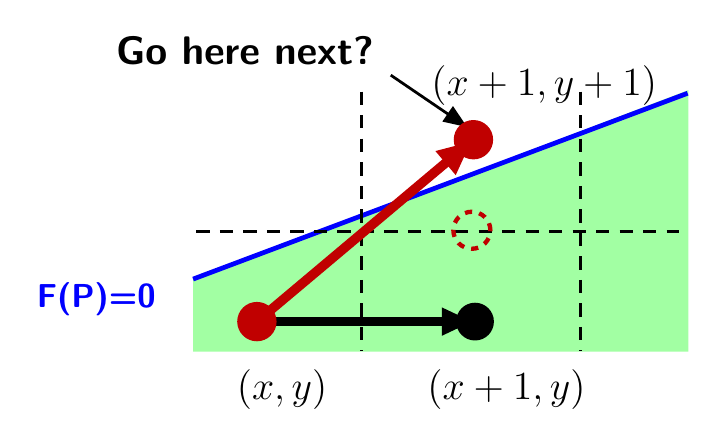
\begin{tikzpicture}[x=1cm,y=1cm]
  \fill[figgreen] (2.94,2.37) -- (9.23,4.77) -- (9.23,1.45) -- (2.94,1.45) -- cycle;
  \draw[blue,line width=0.06cm] (2.94,2.37) -- (9.22,4.73);
  \draw[line width=0.04cm,dash pattern=on 4.8pt off 3.7pt] (5.075,4.75) -- (5.075,1.46);
  \draw[line width=0.04cm,dash pattern=on 4.8pt off 3.7pt] (7.855,4.75) -- (7.855,1.46);
  \draw[line width=0.04cm,dash pattern=on 4.8pt off 3.7pt] (2.98,2.975) -- (9.11,2.975);
  \draw[line width=0.12cm] (3.75,1.83) -- (6.14,1.83);
  \fill (6.10,2.01) -- (6.48,1.83) -- (6.10,1.65) -- cycle;
  \draw[figred,line width=0.12cm] (3.75,1.83) -- (6.20,3.89);
  \fill[figred] (6.017,3.996) -- (6.468,4.113) -- (6.275,3.690) -- cycle;
  \draw[line width=0.035cm] (5.45,4.96) -- (6.20,4.45);
  \fill (6.240,4.568) -- (6.42,4.30) -- (6.105,4.370) -- cycle;
  \fill[figred] (3.75,1.83) circle (0.25);
  \fill (6.52,1.83) circle (0.24);
  \fill[figred] (6.50,4.14) circle (0.25);
  \draw[figred,line width=0.055cm,dash pattern=on 2.6pt off 2.6pt] (6.48,2.99) circle (0.235);
  \node at (4.07,0.97) {\Large$(x,y)$};
  \node at (6.92,0.97) {\Large$(x+1,y)$};
  \node at (7.40,4.83) {\Large$(x+1,y+1)$};
  \node at (3.60,5.27) {\Large\sffamily\bfseries Go here next?};
  \node[blue] at (1.71,2.12) {\large\sffamily\bfseries F(P)=0};
\end{tikzpicture}
\end{center}

要想避免浮点数得到隐函数，可以借用直线上已知点P,关注直线法向量和$\overrightarrow{PP_0}$的点乘结果，判断位置，从而构造出隐函数$F(P)$

\definecolor{figpink}{RGB}{255,197,207}

\begin{center}
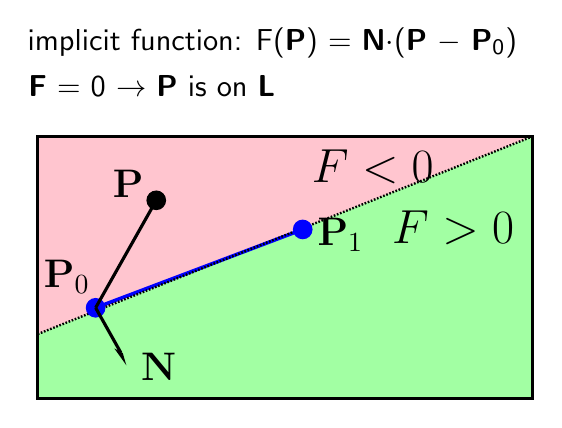
\begin{tikzpicture}[x=1cm,y=1cm]
  \fill[figpink] (1.495,1.566) -- (1.495,4.075) -- (7.775,4.075) -- cycle;
  \fill[figgreen] (1.495,1.566) -- (7.775,4.075) -- (7.775,0.745) -- (1.495,0.745) -- cycle;
  \draw[line width=0.04cm] (1.495,0.745) rectangle (7.775,4.075);
  \draw[blue,line width=0.045cm] (2.23,1.90) -- (4.86,2.895);
  \draw[line width=0.03cm,dash pattern=on 0.6pt off 0.6pt] (1.495,1.566) -- (7.775,4.075);
  \fill[blue] (2.23,1.90) circle (0.125);
  \fill[blue] (4.86,2.895) circle (0.125);
  \draw[line width=0.04cm] (2.23,1.90) -- (3.00,3.265);
  \fill (3.00,3.265) circle (0.125);
  \draw[line width=0.04cm] (2.23,1.90) -- (2.55,1.33);
  \fill (2.468,1.383) -- (2.62,1.17) -- (2.574,1.327) -- cycle;
  \node at (2.645,3.47) {\Large$\mathbf{P}$};
  \node at (1.865,2.29) {\Large$\mathbf{P}_0$};
  \node at (5.34,2.83) {\Large$\mathbf{P}_1$};
  \node at (3.03,1.155) {\Large$\mathbf{N}$};
  \node at (5.75,3.695) {\LARGE$F<0$};
  \node at (6.77,2.92) {\LARGE$F>0$};
  \node[anchor=west,inner sep=0pt] at (1.36,5.265) {\fontsize{11.2}{13.2}\selectfont\sffamily implicit function: F(\textbf{P}) = \textbf{N}$\cdot$(\textbf{P} $-$ \textbf{P}\textsubscript{0})};
  \node[anchor=west,inner sep=0pt] at (1.37,4.715) {\fontsize{11.2}{13.2}\selectfont\sffamily\textbf{F} = 0 $\rightarrow$ \textbf{P} is on \textbf{L}};
\end{tikzpicture}
\end{center}

由于最后只关心和0的关系，所以可以不用归一化直线斜率等信息，直接进行整数运算。由于代入点的时候道理是一样的，可以把斜率乘以2,将向量的增量$(1, \frac{1}{2})$也变成整数进行计算。

最终得到：

\[
F(P) = 2N \cdot (P - P_0)
F(P + \Delta) = F(P) + 2N \cdot \Delta
\]

是一个可迭代的整数运算。从而可以进行循环，得到该运算的代码,借用了点乘来构造方程：

\begin{lstlisting}[style=MyCppStyle]
    int dx = 2*(x1-x0),
    int dy = 2*(y1-y0);
    int dydx = dy-dx;
    F = 0 + dy – dx/2;
    for (x=x0 ; x<=x1 ; x++) {
        draw_pixel(x, y);
        if (F<0) F += dy;
        else {y++; F += dydx;}
}
\end{lstlisting}

\subsubsection{曲线的绘制}

上述算法只要知道了曲线方程的隐函数表示，可以用类似比较大小的手段画曲线，但是由于二次甚至三次方程的求解较为困难，所以很难优化到整数级别的运算难度。

对于圆这样的图形，每一次迭代可以同时画出对称的8个点，实现类似于并行计算的效果。

\begin{lstlisting}[style=MyCppStyle]
    void draw_circle(int radius) 
    {
        int x = 0, y = radius;
        int d = 3-2*radius;
        while (y>x) {
            if (d<0) /* select East point next */
            d += 4*x + 6;
            else { /* select South-East point next */
            d += 4*(x-y) + 10;
            y--;}
        x++;
        draw_8_pts(x,y); /* draws point in each octant */
        }
}
\end{lstlisting}

\paragraph{曲线的表示方法}

更加普遍的曲线绘制方法取决于曲线的表示方式，主要有两种：显式表示和隐式表示。

\begin{itemize}
    \item Explicit显式表达：函数表达式$y= f(x)$,可以用带入的方法快速得到复杂曲线。
    \item Implicit隐式表达：分形曲线，Signed Distance Fuction，解析几何方程
\end{itemize}

在曲线基础绘制中的一个主题是曲线的参数方程表示（Parametric）。回顾圆的参数方程：
\[
\begin{cases}
    x(t) = r \cos t,\\
    y(t) = r \sin t
\end{cases}
\]

可以看到曲线方程具有较好的表示形式和稳定性，可以相应地降低计算量，表示的曲线范围也更广。并且数学上参数曲线的微分容易计算。

\[
\mathbf r'(t)
=
\frac{d\mathbf r}{dt}
=
\begin{bmatrix}
x'(t)\\
y'(t)\\
z'(t)
\end{bmatrix}.
\]

在明确了表示方法之后，我们可以发现曲线的绘制不能用直接的lagarange插值法得到高阶多项式，因为这样会使得计算难度过大。容易想到可以分段计算拼成光滑情况的多项式(Piecewise Fuctions),平衡连续性和可控性。
由此发展出多种插值方法：

\paragraph{Linear Interpolation}

线性插值在两个点之间直接绘制直线，一个线性插值函数记作lerp，则：

\[
lerp(t) = (1 - t) u_0 + t u_1
\]

根据上述计算，构造插值的Basis Fuction，将一个图像上所有点的插值规则集合在同样一个函数里面。已知插值方程为：

\definecolor{lerpblue}{RGB}{135,165,217}   % 基函数三角形填充（蓝）
\definecolor{lerpgreen}{RGB}{197,222,182}  % 基函数三角形填充（绿）
\definecolor{lerpoverlap}{RGB}{126,168,158}% 两个三角形重叠处
\definecolor{lerpdotblue}{RGB}{68,114,196} % 采样点 $y_i$
\definecolor{lerpdotgreen}{RGB}{112,173,71}% 采样点 $y_{i+1}$
\definecolor{lerpdashblue}{RGB}{48,78,130}
\definecolor{lerpdashgreen}{RGB}{52,77,37}

\begin{center}
\begin{minipage}[c]{6.9cm}
  \centering
  % 坐标按原图像素给出，x/y 方向各按 0.0141cm/px 缩放（y 轴向下）
  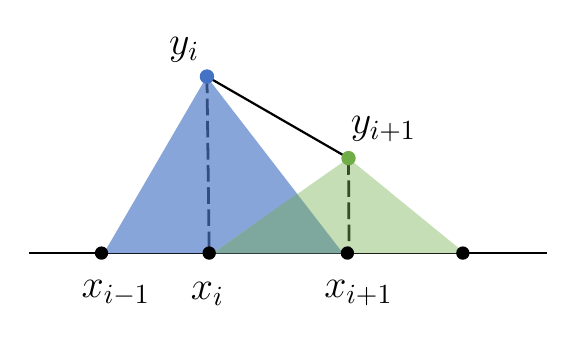
\begin{tikzpicture}[x=0.0141cm,y=-0.0141cm]
    % 横轴
    \draw[line width=0.8pt] (18,243) -- (485,243);
    % 两个基函数的三角形（先蓝后绿，重叠区域再用混合色覆盖）
    \fill[lerpblue]    (178.3,84)    -- (85.7,243)  -- (300.9,243) -- cycle;
    \fill[lerpgreen]   (306,157.5)   -- (410.7,243) -- (184.2,243) -- cycle;
    \fill[lerpoverlap] (259.6,189.5) -- (184.2,243) -- (300.9,243) -- cycle;
    % 由采样点向横轴作的两条虚竖线
    \draw[lerpdashblue,line width=1pt,dash pattern=on 6pt off 2pt]  (178.5,84) -- (180.5,243);
    \draw[lerpdashgreen,line width=1pt,dash pattern=on 6pt off 2pt] (306,157.5) -- (306.5,243);
    % 连接两个采样点的直线
    \draw[line width=0.8pt] (178.5,84) -- (306,157.5);
    % 横轴上的结点与两个采样点
    \fill (83.5,243)  circle[radius=0.0846cm];
    \fill (180.5,243) circle[radius=0.0846cm];
    \fill (305,243)   circle[radius=0.0846cm];
    \fill (409,243)   circle[radius=0.0846cm];
    \fill[lerpdotblue]  (178.5,84)    circle[radius=0.0917cm];
    \fill[lerpdotgreen] (306,157.5)   circle[radius=0.0917cm];
    % 标注
    \node at (158,59.5)  {\Large$y_i$};
    \node at (337.5,131) {\Large$y_{i+1}$};
    \node at (96.5,279)  {\Large$x_{i-1}$};
    \node at (179,280)   {\Large$x_i$};
    \node at (315,279)   {\Large$x_{i+1}$};
  \end{tikzpicture}
\end{minipage}\hspace{1.1cm}%
\begin{minipage}[c]{6.9cm}
  \centering\large\renewcommand{\arraystretch}{0.6}
  $\textstyle y = \frac{x_{i+1}-x}{x_{i+1}-x_i}y_i + \frac{x-x_i}{x_{i+1}-x_i}y_{i+1}$
  \\[1.7em]
  $\textstyle B_i(x) = \begin{cases}
      \frac{x-x_{i-1}}{x_i-x_{i-1}}, & x \in [x_{i-1},x_i] \\[-2.5pt]
      \frac{x_{i+1}-x}{x_{i+1}-x_i}, & x \in [x_i,x_{i+1}] \\[-2.5pt]
      0, & \text{else}
  \end{cases}$
\end{minipage}
\end{center}

基函数是插值问题中更加广泛的概念，对于一个基函数$B_i(x)$,满足以下要求（公理）：

\[
B_i(x_j) = \delta_{ij} = 
\begin{cases}
    1, i = j,\\
    0, i \not = j
\end{cases}
\]

\paragraph{Bezier Curve Interpolation}

1962年，法国雷诺汽车公司（Renault）的工程师Pierre Bezier提出了一种新的曲线表示方式：给定起点$u_0$与终点$u_1$，再补充若干个额外的控制点，就能让一条光滑曲线被这些控制点"牵引"着从$u_0$走到$u_1$。

\definecolor{bezpt}{RGB}{255,0,0}        % 端点 $u_0,u_1$
\definecolor{bezctrl}{RGB}{0,0,255}      % 控制点 $t_0$
\definecolor{bezlerp}{RGB}{71,219,205}   % 中间点 $a_0,a_1$ 与构造边
\definecolor{bezb}{RGB}{112,48,160}      % 点 $b$
\definecolor{bezorange}{RGB}{197,90,17}  % 橙色标注与箭头
\definecolor{bezcurve}{RGB}{242,196,132} % 二次 Bezier 曲线
\definecolor{bezhull}{RGB}{237,125,49}   % 凸包图中的三次 Bezier 曲线
\definecolor{bezb1}{RGB}{47,189,253}     % $(1-t)^3$
\definecolor{bezb2}{RGB}{242,163,241}    % $3t(1-t)^2$
\definecolor{bezb3}{RGB}{77,219,206}     % $3t^2(1-t)$
\definecolor{bezb4}{RGB}{244,180,84}     % $t^3$

\subparagraph{生成与动机}

先考察最简单的配置：除两个端点之外只多给一个控制点$t_0$。构造完全建立在上一节的lerp之上，先在两条边上各取一个按同一参数$t$插值出来的中间点：

\[
a_0 = lerp(u_0,t_0,t) = (1-t)u_0 + t\,t_0, \qquad
a_1 = lerp(t_0,u_1,t) = (1-t)t_0 + t\,u_1
\]

再把$a_0,a_1$当作一对新的端点，做一次同样的插值：

\[
b = lerp(a_0,a_1,t) = (1-t)a_0 + t\,a_1
\]

固定$t$时$b$是曲线上的一个点；让$t$从0连续变到1，$b$扫过的轨迹就是所要求的那条曲线。下图取$t=0.6$：三条构造边上的花括号标注的其实是同一件事——每一轮插值得到的点都把所在的那条边按$t:(1-t)$分成两段，所以三个花括号都写$t=0.6$。可以看到$b$恰好落在曲线上。

\begin{center}
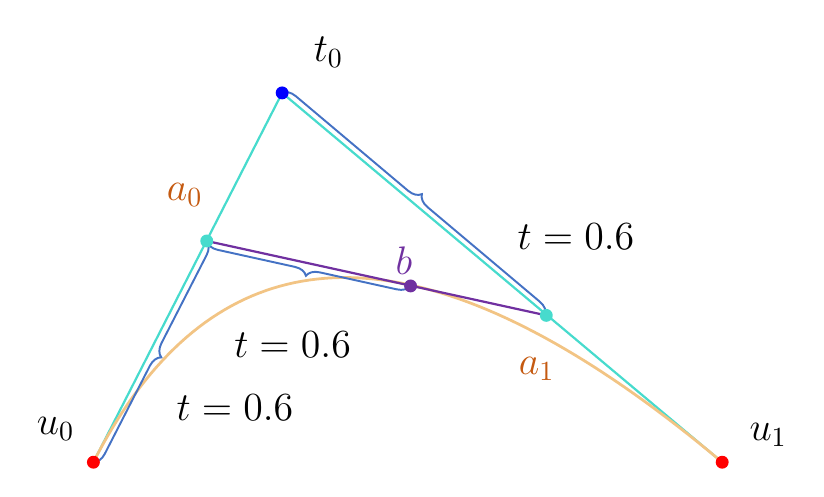
\begin{tikzpicture}[x=0.0114cm,y=-0.0114cm]
  % 坐标按课件原图像素给出，x/y 方向各按 0.0114cm/px 缩放（y 轴向下）
  % 两条构造边 u0-t0-u1
  \draw[bezlerp,line width=0.8pt] (108.1,1020.9) -- (318.4,609.4) -- (808.7,1020.9);
  % 二次 Bezier 曲线：(1-t)^2 u0 + 2t(1-t) t0 + t^2 u1
  \draw[bezcurve,line width=1pt]
    plot[domain=0:1,samples=80,variable=\t]
    ({(1-\t)*(1-\t)*108.1 + 2*\t*(1-\t)*318.4 + \t*\t*808.7},
     {(1-\t)*(1-\t)*1020.9 + 2*\t*(1-\t)*609.4 + \t*\t*1020.9});
  % a0-a1 连线，b 落在其上
  \draw[bezb,line width=0.8pt] (234.4,774.4) -- (612.7,857.3);
  % 三条构造边上的花括号：每轮插值都把所在的边按 t:(1-t) 分段，故均标 t=0.6
  \draw[lerpdotblue,line width=0.7pt,decorate,
        decoration={brace,amplitude=0.16cm,mirror}]
        (108.1,1020.9) -- (234.4,774.4);
  \draw[lerpdotblue,line width=0.7pt,decorate,
        decoration={brace,amplitude=0.16cm}]
        (318.4,609.4) -- (612.7,857.3);
  \draw[lerpdotblue,line width=0.7pt,decorate,
        decoration={brace,amplitude=0.16cm,mirror}]
        (234.4,774.4) -- (461.5,824.5);
  % 端点、控制点与三个中间点
  \fill[bezpt]   (108.1,1020.9) circle[radius=0.082cm];
  \fill[bezpt]   (808.7,1020.9) circle[radius=0.082cm];
  \fill[bezctrl] (318.4,609.4)  circle[radius=0.082cm];
  \fill[bezlerp] (234.4,774.4)  circle[radius=0.082cm];
  \fill[bezlerp] (612.7,857.3)  circle[radius=0.082cm];
  \fill[bezb]    (461.5,824.5)  circle[radius=0.082cm];
  % 标注
  \node at (66,984)             {\Large$u_0$};
  \node at (370,564)            {\Large$t_0$};
  \node at (860,991)            {\Large$u_1$};
  \node[bezorange] at (210,723) {\Large$a_0$};
  \node[bezorange] at (602,917) {\Large$a_1$};
  \node[bezb] at (454,796)      {\Large$b$};
  \node[anchor=west] at (190,960) {\Large$t=0.6$};
  \node[anchor=west] at (570,770) {\Large$t=0.6$};
  \node at (330,890)              {\Large$t=0.6$};
\end{tikzpicture}
\end{center}

阶数提高时做法没有任何变化，只是"更多的线、更多次lerp"：控制点增加到两个就是二次（square）Bezier曲线，增加到三个就是三次（cubic）Bezier曲线。一条三次Bezier有两个控制点，需要$3+2+1$次lerp——每做完一轮插值，点的个数就减少一个，所以这个过程天然是递推的。

\subparagraph{De Casteljau 迭代算法}

上面这套做法称为De Casteljau算法（德卡斯特里奥）。给定参数$t$，它只有两步：

\begin{enumerate}
    \item 对每一对相邻的控制点，按参数$t$计算它们的线性插值；
    \item 用插值得到的结果作为新的控制点集合，重复上一步。
\end{enumerate}

当控制点只剩下一个时递归终止，剩下的这个点就是参数$t$处的曲线上的点。写成递归函数即：

\begin{lstlisting}[style=MyCppStyle, language=Python]
def bezier_recursive(points, t):
    # only one point left: recursion ends, this is the point on the curve
    if len(points) == 1:
        return points[0]

    # otherwise: linear interpolation between every pair of neighbours
    new_points = []
    for i in range(len(points) - 1):
        # linear interpolation: P = (1 - t) * P1 + t * P2
        new_points.append((1 - t) * points[i] + t * points[i + 1])

    # recurse on the reduced set of control points
    return bezier_recursive(new_points, t)
\end{lstlisting}

把lerp的系数逐层乘开，就得到同一个结果的解析形式。以二次曲线为例（控制点在这里记作$c_0$，也就是上文的$t_0$）：

\[
b = (1-t)a_0 + t\,a_1
  = (1-t)^2u_0 + 2t(1-t)c_0 + t^2u_1
\]

中间项$2t(1-t)$的系数2来自两条路径的合并：$c_0$既可以在$a_0$一侧乘$(1-t)$、再在$a_1$一侧乘$t$得到，也可以反过来。把每一条路径上的因子都画出来，就得到下面这棵树——蓝色箭头表示乘$(1-t)$，橙色箭头表示乘$t$，从$b$出发走到哪个端点，乘出来的就是那个端点的权重：

\begin{center}
\begin{tikzpicture}[x=0.0105cm,y=-0.0105cm,>=latex,every node/.style={font=\large}]
  % 第 0 层
  \node at (80,1086)  {$\color{bezb}b$};
  \node at (133,1077) {$1$};
  % 第 1 层
  \node[bezorange] at (198,1002) {$a_0$};
  \node at (352,986)  {$1-t$};
  \node[bezorange] at (204,1157) {$a_1$};
  \node at (342,1177) {$t$};
  % 第 2 层
  \node at (481,905)  {$u_0$};
  \node at (696,891)  {$(1-t)^2$};
  \node[bezorange] at (516,1012) {$c_0$};
  \node at (711,1083) {$2t(1-t)$};
  \node[bezorange] at (485,1105) {$c_0$};
  \node at (455,1253) {$u_1$};
  \node at (678,1274) {$t^2$};
  % 箭头：蓝 = *(1-t)，橙 = *t
  \draw[->,lerpdotblue,line width=0.7pt] (165,1077) -- (258,994);
  \draw[->,bezorange,line width=0.7pt]   (165,1085) -- (258,1157);
  \draw[->,lerpdotblue,line width=0.7pt] (437,995)  -- (550,898);
  \draw[->,bezorange,line width=0.7pt]   (437,1008) -- (560,1065);
  \draw[->,lerpdotblue,line width=0.7pt] (437,1175) -- (560,1105);
  \draw[->,bezorange,line width=0.7pt]   (437,1188) -- (560,1268);
  % 图例
  \node at (338,1400) {$*(1-t)$};
  \node at (555,1400) {$*t$};
  \draw[->,lerpdotblue,line width=0.7pt] (275,1435) -- (410,1435);
  \draw[->,bezorange,line width=0.7pt]   (495,1435) -- (630,1435);
\end{tikzpicture}
\end{center}

值得强调的是，尽管Bezier曲线有解析表达式，实际绘制时仍然使用De Casteljau算法：与解析表达式相比，它更加高效、数值也更加稳定。

\subparagraph{解析表示：Bernstein多项式与杨辉三角}

把上面的过程继续推到三次，四个权重分别是

\[
(1-t)^3,\qquad 3t(1-t)^2,\qquad 3t^2(1-t),\qquad t^3
\]

系数$1,3,3,1$恰好是杨辉三角（Pascal's triangle）的一行：

\[
\begin{array}{c}
1\\[1pt] 1\quad 1\\[1pt] 1\quad 2\quad 1\\[1pt] 1\quad 3\quad 3\quad 1\\[1pt]
1\quad 4\quad 6\quad 4\quad 1\\[1pt] 1\quad 5\quad 10\quad 10\quad 5\quad 1\\[1pt]
1\quad 6\quad 15\quad 20\quad 15\quad 6\quad 1\\[1pt]
1\quad 7\quad 21\quad 35\quad 35\quad 21\quad 7\quad 1
\end{array}
\]

因此这些权重函数也叫Bernstein多项式，一般地有

\[
B(t) = \sum_{k}\binom{n}{k}t^k(1-t)^{n-k}
\]

把权重乘回控制点，就得到$n$次Bezier曲线的解析表达式：

\[
b(t) = \sum_{k=0}^{n}\binom{n}{k}t^k(1-t)^{n-k}u_k,\qquad k = 0,1,\dots,n
\]

三次的情形写开就是

\[
b(t) = (1-t)^3u_0 + 3t(1-t)^2u_1 + 3t^2(1-t)u_2 + t^3u_3
\]

把它整理成矩阵乘积，可以更清楚地看到"权重"与"控制点"是分离的两部分：

\[
b(t) = \boldsymbol\tau^{\mathsf T}M_B\mathbf u = B(t)^{\mathsf T}\mathbf u
\]

其中

\[
\boldsymbol\tau = \begin{bmatrix}1\\t\\t^2\\t^3\end{bmatrix},\qquad
M_B = \begin{bmatrix}
    1 & 0 & 0 & 0\\
    -3 & 3 & 0 & 0\\
    3 & -6 & 3 & 0\\
    -1 & 3 & -3 & 1
\end{bmatrix},\qquad
B(t) = \begin{bmatrix}
    (1-t)^3\\ 3t(1-t)^2\\ 3t^2(1-t)\\ t^3
\end{bmatrix},\qquad
\mathbf u = \begin{bmatrix}u_0\\u_1\\u_2\\u_3\end{bmatrix}
\]

$M_B$是只与次数有关的常数矩阵，$B(t)$则只与参数$t$有关，它被称为混合函数（blending functions）。四条混合函数的图像如下。

\begin{center}
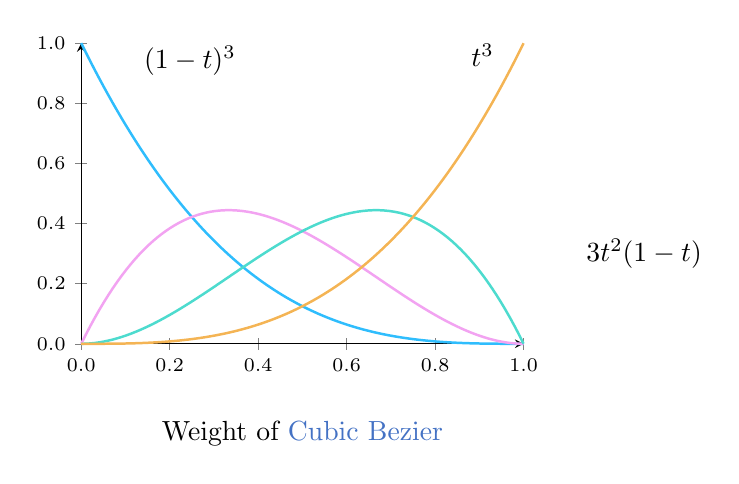
\begin{tikzpicture}
\begin{axis}[
    width=7.2cm, height=5.4cm,
    xmin=0, xmax=1, ymin=0, ymax=1,
    xtick={0,0.2,0.4,0.6,0.8,1}, ytick={0,0.2,0.4,0.6,0.8,1},
    xticklabel style={/pgf/number format/fixed, /pgf/number format/zerofill, /pgf/number format/precision=1},
    yticklabel style={/pgf/number format/fixed, /pgf/number format/zerofill, /pgf/number format/precision=1},
    tick label style={font=\scriptsize},
    axis lines=left,
    clip=false,
    every axis plot/.append style={line width=0.9pt},
]
  \addplot[domain=0:1,samples=100,bezb1]{(1-x)^3};
  \addplot[domain=0:1,samples=100,bezb2]{3*x*(1-x)^2};
  \addplot[domain=0:1,samples=100,bezb3]{3*x^2*(1-x)};
  \addplot[domain=0:1,samples=100,bezb4]{x^3};
  \node[anchor=west] at (axis cs:0.12,0.94) {$(1-t)^3$};
  \node[anchor=west] at (axis cs:0.86,0.96) {$t^3$};
  \node[anchor=west] at (axis cs:1.12,0.30) {$3t^2(1-t)$};
  \node at (axis cs:0.5,-0.30) {Weight of \textcolor{lerpdotblue}{Cubic Bezier}};
\end{axis}
\end{tikzpicture}
\end{center}

至此可以把Bezier曲线和上一节的lerp放在一起看：两者都是控制点的加权和，区别只在于权重函数。lerp的权重是$(1-t)$与$t$——也就是本节开头画过的那两个三角形；三次Bezier的权重则是上面这四条曲线。

\subparagraph{性质}

混合函数在端点处的取值决定了曲线在两个端点处的行为。对$n$次Bezier曲线，

\[
B'(0) = n(u_1-u_0), \qquad B'(1) = n(u_n-u_{n-1})
\]

也就是说，曲线在$u_0$处的切向就是$u_0\to u_1$的方向（这里的$u_1$指的是紧邻$u_0$的那个控制点）。借助这条性质可以光滑地拼接两条Bezier曲线：只要让接点两侧的一对控制点关于接点中心对称即可。

另一条性质来自Bernstein多项式本身：它保证了Bezier曲线一定落在其控制点的凸包（convex hull）之内——虽然这并不是最紧的界。因此即使我们不存储曲线上的所有数据，也不会偏离控制点太远。

\begin{center}
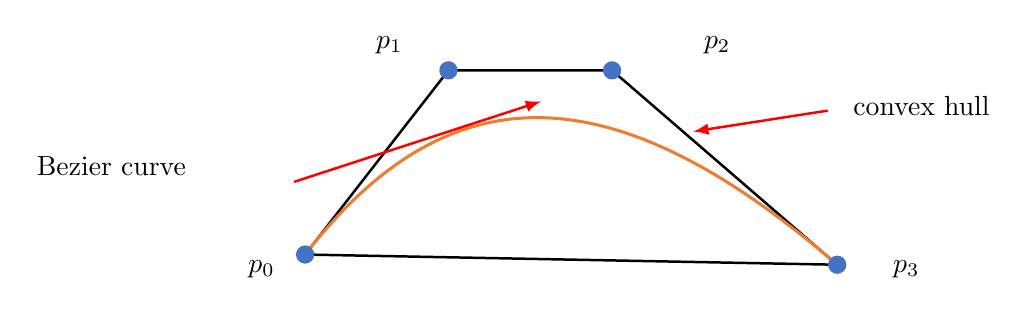
\begin{tikzpicture}[x=0.0078cm,y=-0.0078cm]
  % 控制多边形（凸包的边）
  \draw[line width=0.9pt] (482.8,1288.4) -- (716.2,988.4) -- (982.8,988.4) -- (1349.5,1305.0) -- cycle;
  % 以 p0..p3 为控制点的三次 Bezier 曲线
  \draw[bezhull,line width=1.1pt]
    plot[domain=0:1,samples=80,variable=\t]
    ({(1-\t)^3*482.8 + 3*\t*(1-\t)^2*716.2 + 3*\t*\t*(1-\t)*982.8 + \t*\t*\t*1349.5},
     {(1-\t)^3*1288.4 + 3*\t*(1-\t)^2*988.4 + 3*\t*\t*(1-\t)*988.4 + \t*\t*\t*1305.0});
  % 四个控制点
  \fill[lerpdotblue] (482.8,1288.4)  circle[radius=0.116cm];
  \fill[lerpdotblue] (716.2,988.4)   circle[radius=0.116cm];
  \fill[lerpdotblue] (982.8,988.4)   circle[radius=0.116cm];
  \fill[lerpdotblue] (1349.5,1305.0) circle[radius=0.116cm];
  % 红色指示箭头
  \draw[->,bezpt,line width=0.9pt,>=latex] (465,1170) -- (867,1039);
  \draw[->,bezpt,line width=0.9pt,>=latex] (1334,1054) -- (1115,1088);
  % 标注
  \node[anchor=west] at (30,1144)   {Bezier curve};
  \node[anchor=west] at (1360,1046) {convex hull};
  \node at (620,948)   {$p_1$};
  \node at (1154,948)  {$p_2$};
  \node at (412,1312)  {$p_0$};
  \node at (1462,1312) {$p_3$};
\end{tikzpicture}
\end{center}

\paragraph{B-splines}

B-样条曲线的绘制，主要算法是求解基函数。与Bezier的基函数是伯恩斯坦多项式不同，B-splines曲线不设定两个控制点，而是通过多次的插值和直线向量的迭代一次得到1阶到n阶基函数。

\subparagraph{数学本质}

B-spline曲线把分段参数曲线写成控制点的加权和：

\[
\mathbf b(t) = \sum_{i=0}^{m}N_{i,n}(t)\mathbf P_i,\qquad \mathbf P = \{\mathbf P_0,\mathbf P_1,\dots,\mathbf P_m\}
\]

与Bezier的差别在于基函数的支撑集。Bernstein多项式在整个$[0,1]$上都非零，所以一个控制点影响整条曲线，而片与片之间又毫无关联；B-spline的基函数$N_{i,n}$只在$[t_i,t_{i+p+1}]$上非零，控制点因此只有局部影响，移动一个点只改动相邻的少数几段。基函数还满足单位分解

\[
\sum_i N_{i,p}(t) = 1,\qquad t\in[0,1]
\]

所以曲线仍然落在控制点的凸包之内。所有基函数的定义域取$[u_0,u_m]$，通常令$u_0=0,\ u_m=1$，即闭区间$[0,1]$。

\subparagraph{算法：Cox--de Boor递推}

基函数并不直接写出解析式，而是从0阶开始逐阶递推得到，这就是Cox--de Boor递推：

\[
N_{i,0}(t) = \begin{cases}1, & t_i\le t<t_{i+1},\\ 0, & \text{otherwise},\end{cases}
\]

\[
N_{i,p}(t) = \frac{t-t_i}{t_{i+p}-t_i}N_{i,p-1}(t) + \frac{t_{i+p+1}-t}{t_{i+p+1}-t_{i+1}}N_{i+1,p-1}(t)
\]

0阶基函数是分段常数（方波），1阶是三角波，阶数继续升高曲线逐渐光滑：$p$阶基函数是$C^{p-1}$的。曲线的形状完全由节点序列（knot sequence）决定，节点均匀时称为均匀B-spline。求值时给定$t$只有$p+1$个基函数非零，逐层递推即可，代价与总控制点数$m$无关，这也是它比Bezier更适合表示长曲线的原因。

\subparagraph{Cubic B-spline}

取$p=3$。每条基函数跨越4个节点区间，于是$[p_{i-1},p_i]$这一段只由4个控制点决定：

\[
\mathbf p = [p_{i-2},p_{i-1},p_i,p_{i+1}]^{\mathsf T}
\]

令$u = (t-t_i)/(t_{i+1}-t_i)$，这一段可以写成与三次Bezier完全平行的形式

\[
p(u) = \boldsymbol\tau^{\mathsf T}M_S\mathbf p = \mathbf b(u)^{\mathsf T}\mathbf p
\]

其中

\[
\mathbf b(u) = \frac16\begin{bmatrix}(1-u)^3\\ 4-6u^2+3u^3\\ 1+3u+3u^2-3u^3\\ u^3\end{bmatrix},\qquad
M_S = \frac16\begin{bmatrix}
    1 & 4 & 1 & 0\\
    -3 & 0 & 3 & 0\\
    3 & -6 & 3 & 0\\
    -1 & 3 & -3 & 1
\end{bmatrix}
\]

$M_S$的每一行都不止一个非零元，一条基函数要跨过4段，这正对应它的局部支撑。三次B-spline具有$C^{n-1}=C^2$连续性：函数值、一阶导与二阶导在连接点都连续，而且不需要像自然三次样条那样解方程组。

绘制时使用滑动窗口（sliding window）：每加入一个新的控制点，$\mathbf p$与$M_S$就向前滑动一段。每一段还可以改写成一条三次Bezier曲线，由

\[
p(u) = \boldsymbol\tau^{\mathsf T}M_BP_B = \boldsymbol\tau^{\mathsf T}M_SP_S
\]

得到$P_B = M_B^{-1}M_SP_S$，也就是把4个B-spline控制点换算成4个Bezier控制点，之后就能直接用De Casteljau算法绘制。

把参数推广到两个方向就得到B-spline曲面（patches）：

\[
p(u,v) = \sum_{i=0}^{3}\sum_{j=0}^{3}b_i(u)b_j(v)p_{ij} = \boldsymbol\tau^{\mathsf T}M_SPM_S^{\mathsf T}\boldsymbol\tau
\]

形式上与Bezier曲面一样是16个控制点的加权和，但每片patch只覆盖定义域的$1/9$。

\subsubsection{凸多边形的绘制}

凸多边形的判断并不容易，所以主要关注绘制三角形的算法。算法的基本原理是用一条直线自上而下进行扫描，一条一条地扫描，左右两侧的点由前述算法逐步确定。

对于一般的多边形可以进行三角化分割，归结到前面的算法。

具体来说，这套扫描转换流程需要依次完成以下几件事：先找出多边形的最高顶点与最低顶点，由此确定扫描线的起止范围；再把多边形的边沿着左右两侧分别组织成边表（左侧链与右侧链），按扫描线自上而下逐条处理；由于凸多边形每条扫描线只与边界相交两次，每条扫描线上只有一个待填充的区间（span），求出区间左右端点的横坐标$x_L, x_R$之后（端点也可以借助Bresenham算法顺带求出），把两者之间的像素全部填上颜色即可。相邻两条扫描线的端点之间满足

\[
x_L \mathrel{+}= \frac{dx_L}{dy_L}, \qquad x_R \mathrel{+}= \frac{dx_R}{dy_R}
\]

所以端点的推进同样是增量式的，与前面画直线的迭代完全一致。

上面这些环节中任何一处处理不当，都会在相邻多边形的公共边上留下痕迹：如果两侧链的取舍或者端点的取整规则不一致，公共边可能被填充两次，也可能一次都没有被填充，于是出现重叠（overlap）或者裂缝（crack）。

\subsubsection{凹多边形与三角化}

凹多边形的麻烦在于一条扫描线与它的交点可能多于两个，“每条扫描线只有一个区间”的前提不再成立。此时的做法是：求出该扫描线与多边形的全部交点，把它们按横坐标从左到右排序，再依次两两配对填充，这就是奇偶规则（parity rule）——排序后第1、2个交点之间是内部，第3、4个交点之间也是内部，奇数号交点为入点，偶数号交点为出点。也就是说，从某点向左引出的射线与多边形边界的交点个数为奇数时该点在内部，为偶数时在外部。

另一条思路是三角化（triangulation）：先把凹多边形分割成若干个三角形，再对每个三角形套用前面凸多边形的扫描转换流程。这样做的好处是内层循环永远是简单的单区间填充，不需要求交排序与奇偶判断；而只要共享同一条边的两个三角形对这条边的取整规则保持一致，拼接处既不会出现裂缝也不会重叠。代价是需要额外做一步三角化（对简单多边形可以用耳切法ear clipping，逐个切掉凸耳）。两种做法本质上是在“逐扫描线求交排序”与“事先分割、简化内层循环”之间做取舍。

\subsection{Warping}
（课堂上面只是做了科普，真正的内容远远少于下面的表述，表述是AI完成的）

在Image Warping中，进行图像的变形操作，比如对图片进行拉伸，扭曲，控制。具体而言就是整体或者局部的坐标系变换。

常见的方法是网格方法，将空间的网格进行拖动，挪移等操作。在PS软件中，实际上操作光标的中心是一个kernel，以相同的幅度和倍率进行平移和非线性形变。

对于RGB图像，一般会进行颜色插值，四边形和三角形的不同网格表示会导向不同的插值方法，非线性插值和线性插值都会出现在Warping中。

具体地，可以把图像看成定义在参数域上的函数：源图的一个正方形区域由四个角点参数化——左上$(u_0,v_0)$、右上$(u_1,v_0)$、左下$(u_0,v_1)$、右下$(u_1,v_1)$，Warping就是把这个参数正方形映射成目标图中的任意四边形，正方形的四个角落到四边形的四个角上，源图里的参数点$(u_i,v_j)$则落到四边形中对应的位置。图中的向量$\boldsymbol{u}$表示水平方向的映射，整张图可以理解为参数域到目标域的一次坐标变换，四边形的情形常取双线性映射，更一般（带透视）的情形则是单应（homography）变换。

实现上通常采用反向映射（inverse mapping）：遍历目标图像的每一个像素，用逆变换求出它在源图中对应的参数坐标$(u_i,v_j)$，再按这个坐标到源图里取样。之所以不反过来做正向映射（把源图的每个像素搬到目标位置），是因为正向映射下目标像素未必被覆盖，结果会出现空洞（holes），而多个源像素又可能落到同一个目标像素上造成重叠。

Warping的典型用途是几何矫正：把倾斜拍摄的画面（仰拍的埃菲尔铁塔，或者从侧面拍下来的蒙娜丽莎）重新映射回正视图，也就是所谓的keystone矫正；也可以在图像上覆盖一张控制网格，通过拖动网格的顶点做局部的非线性形变，这与PS里的变形/液化工具是同一个思路。

颜色插值的问题随之而来。把由两个三角形拼成的正方形（用红绿渐变示意）warp成三角形时，如果直接在屏幕空间对纹理坐标或者颜色做线性插值，得到的是“非透视校正”的结果：原本笔直的三角形公共边在结果图里会弯成一条曲线，两块三角形的拼接处发生错位，渐变也随之失真。原因是透视投影下屏幕上的等距并不对应纹理上的等距，参数坐标要先除以深度（齐次坐标里的$w$）才是线性的。正确的做法是透视校正插值（perspective-correct interpolation）：对$u/w$、$v/w$、$1/w$分别做线性插值，最后相除还原出$u,v$，这样三角形的公共边才会保持笔直。

\subsection{反走样（Anti aliasing）}

这一部分是图像处理中反走样的知识。图像发生走样的原因是进行采样的时候精度不够，有一些信息丢失了，因此导致图像模糊，变形。

\subsubsection{走样的发生原因}

对于低频的信息，间隔采样容易保留信息的大体走势。而对于高频的信息，可能采样过程中精度不够，则会发生混叠。划分低频和高频的标准是奈奎斯特准则，即采样频率$f_s$应当大于图像频率$f$的两倍。当$f_s > 2f$时候不发生走样，当$f_s < 2f$时会发生aliasing

下面具体论证Nyquist条件(Nyquist-Shannon Theorem)：

以某一个频率进行采样，等价于频域中脉冲谱和原频谱进行卷积，产生$f_s$间隔的平移周期延拓。在应用中通常只绘一个基本周期内的频谱。如果把频谱在频率平面继续扩展，会沿$f_x$和$f_y$方向以$f_s$为周期重复。如果采样频率过低，则会使卷积之后的高频信号投影到低频的信号空间，两个脉冲发生重叠，在图片上会产生aliasing

以图像为例子，一个高频信号会和低频信号产生相同的采样点，高频信号和低频叠加，就看不出信号的强度了。对于点阵等高频信息，在进行降采样的时候会出现Moore条纹。

\subsubsection{反走样处理·直线}

对于图片的反走样，要进行低通滤波，降低高频信号的比例，滤波结束之后可以办到防止走样。以直线的绘制为例，想要在绘制直线的时候防止图像走样，本质上是使用卷积核进行滤波，让显示直线的不同像素展现出不同的灰度。由于卷积是一个价格昂贵的计算，所以要尽可能降低shading的成本。

卷积核的设计由于直线是一维图像，可以直接把距离定义为信号强度。

\subparagraph{面积采样：求交集面积就是一次卷积}

理想直线是零面积的集合。只在像素中心判断"在不在线上"（0-1采样），等价于用冲激串对连续信号采样：频域中频谱以$f_s$为周期复制，而直线的硬边界含有任意高的频率，复制出来的高频落回低频区，就叠成锯齿。所以关键在于采样之前先做低通。面积采样把这一步直接算进了像素值里，不需要额外增加处理步骤。

给直线一个厚度$w$，得到一条带状区域，记它的指示函数为$S(\xi,\eta)$，像素方框记作$\Pi$，则像素强度取两者的交集面积：

\[
I[i,j] = \iint_{\text{pixel}_{ij}} S(\xi,\eta)\,d\xi\,d\eta = (S*\Pi)(x_i,y_j)
\]

也就是说，求交集面积在数学上就是用$\Pi$这个盒核（box filter）对$S$做一次卷积，再在像素中心取值，滤波与采样合并成了一步。真正生效的核是$\Pi_w*\Pi$，即两个方波的卷积，频域为$\operatorname{sinc}^2$，比单纯的box（频域为$\operatorname{sinc}$，旁瓣衰减只有$1/|f|$）要好，但仍不是陡峭的理想低通。

\subparagraph{一维模型：覆盖率只依赖垂距}

直线是一维图元，这一点让卷积可以大幅简化。一维情形下，宽$w$的带与单位区间的交叠长度只依赖带的中心到区间中心的偏移$d$：

\[
T_w(d) = \max\left(0,\ \min\left(w,\ \frac{1+w}{2}-|d|\right)\right), \qquad \int_{-\infty}^{\infty}T_w(d)\,dd = w
\]

即一个梯形：$|d|\le\frac{1-w}{2}$时饱和在$w$，到$|d| = \frac{1+w}{2}$线性降到零（$w=1$时正好退化成tent）。推广到二维，对直线$y = mx+b$，像素中心到直线的垂距为

\[
d = \frac{|mx_i - y_j + b|}{\sqrt{1+m^2}}
\]

对一条直带（忽略端点与像素角点），覆盖率仍然只由$d$决定。所以"把距离定义为信号强度"并非人为约定，而是因为覆盖率本来就只随垂距变化。注意$T_w$的积分等于$w$而不是1，要当作合法的低通核使用，还需除以$w$归一化。

\subparagraph{加权面积采样}

把盒核换成可自由选择的权重函数$f$，就得到加权面积采样：

\[
I[i,j] = \iint S(\xi,\eta)f(\xi - x_i,\ \eta - y_j)\,d\xi\,d\eta = (S*f)(x_i,y_j)
\]

$f$可以取任何形状，但要满足三条约束：

\begin{enumerate}[nosep]
\item 支撑有限（finite non-zero region）：每个像素只受邻近图元影响，可以局部计算；
\item 随距离单调衰减：越远的图元贡献越小，避免相邻像素互相串色；
\item 全"面积"等于1，即$\iint f = 1$：归一化条件，等价于频域的$F(0,0) = 1$，即直流增益为1。只有这样，一整片纯色区域采样后仍是原来的纯色，不会被压暗或者提亮。
\end{enumerate}

前两条只关乎"合理"，第三条是硬性的。常见的四种核是box、tent（Bartlett）、Gaussian与cone，区别主要在频域的衰减速度：

\[
\text{box}\to\operatorname{sinc}\ (\sim |f|^{-1}),\qquad
\text{tent}\to\operatorname{sinc}^2\ (\sim |f|^{-2}),\qquad
\text{Gaussian}\to\text{Gaussian}
\]

box与tent的传递函数都带旁瓣，截止频率以上的残留会以反相形式混回来，表现为残余走样；Gaussian没有旁瓣、衰减最快，效果最好，代价是支撑无限，实现时必须截断，而截断又会重新引入旁瓣，工程上的取舍就在这里。这也说明加权为什么优于纯面积采样：纯面积用的核是$\Pi_w*\Pi$（$\operatorname{sinc}^2$量级），加权之后可以换成衰减更快的核。

幻灯片上写的是"blackness $=$ area $\times\ f(\text{distance})$"，把精确交集面积与衰减权重分成两项相乘。严格说来加权面积采样是一次卷积$(S*f)$，这个乘积形式是便于逐像素快速求值的近似，方向一致但并不等价。

\subparagraph{与超采样的关系}

每像素做$n\times n$超采样再取平均，

\[
I[i,j] = \lim_{n\to\infty}\frac{1}{n^2}\sum_{k=1}^{n}\sum_{l=1}^{n}S(\xi_k,\eta_l)
\]

正是上面那个积分的黎曼和，$n\to\infty$时收敛到精确值。两条路径的区别在于顺序：面积采样解析地求出积分，滤波在前、采样在后，每像素$O(1)$，但只对能写出解析覆盖率的简单图元（直线、多边形）可行；超采样数值地逼近积分，采样在前、滤波在后，通用于任何图元，代价是$O(n^2)$。这也回应了上面提到的成本问题：直线之所以特殊，正是因为它的覆盖率有闭式解，所以能用面积采样把shading的成本压到最低。

\subsubsection{反走样处理·图像}

由于可能对于一张图片的处理需要多次进行低通滤波，为了提高计算效率，针对砖墙等有纹理的图像，提出MIP map算法，这个算法首先用一个box进行卷积平均，做到1个像素为止，然后把多个部分的压缩情况组合存储起来。经过预先计算形成金字塔之后，根据所需的倍数和核的大小在层间进行线性插值（光栅化）。

\subsubsection{超采样技术}

超采样的kernel有多种格式，指的是在图像的变换中按照高于最终降伏网格的密度进行采样，再把多个值合并成一个值得到灰度。

幻灯片中超级采样（super-sampling）的完整过程分三步：先按屏幕分辨率采样，每个像素只取一个点，直线的取值非黑即白；再提高分辨率采样，采样点变密，直线上出现灰度；最后回到屏幕分辨率，把每个像素内的多个采样值合并成一个值，得到灰度。幻灯片左侧另外给出了源图与目标图的对应关系：目标图中的一个像素（红框）在源图中对应一整块区域，因此需要在该区域内取多个采样点。

幻灯片列出的kernel格式依次是：1 sample，$1\times2$ sample，$2\times1$ sample，Quincunx，$2\times2$ grid，$2\times2$ RGSS，$4\times4$ checker，8 rooks，$4\times4$ grid，$8\times8$ checker，$8\times8$ grid。每一种格式都用图标画出了子采样点在像素内的位置，右侧并排给出该格式绘制同一条直线（一个填充三角形与一个线框三角形）的结果。

\subsubsection{多重采样技术}

多重采样是针对于图形而言的，每个像素布置4个子采样点，像素中心不在三角形内部，但部分子采样点被三角形覆盖，该像素仍然会被标记为需要处理。相对超采样，MSAA对该像素仅仅计算一次，不对每个采样点都进行单独着色，然后计算出结果颜色。

幻灯片对比的前提是普通单采样：单采样只看像素中心是否落在三角形内。

以每个像素布置$2\times2$共4个子采样点为例，幻灯片把像素分成两类：

\begin{itemize}[nosep]
\item 内部像素：4/4被覆盖，着色1次，输出$= C$；
\item 边界像素：像素中心在三角形外，但有3/4的子采样点被覆盖，该像素仍会被标记为需要处理。若无反走样，该像素可能直接被丢弃。
\end{itemize}

边界像素的处理流程分三步：覆盖检测（统计4个子采样点中有3个被覆盖）$\to$只计算一次颜色$C$（对该像素的三角形只着色一次）$\to$按覆盖率混合（根据覆盖率与背景进行颜色混合）。于是覆盖率$= 3/4$，最终颜色$= (3/4)\times C$。

直观理解：三角形内部的处理方式几乎与单采样相同；三角形边界则根据子采样覆盖比例平滑边缘。MSAA在边界处效果接近SSAA，但着色开销更低。

MSAA与SSAA的对比：SSAA每个子采样点都单独着色，质量高，开销大；MSAA主要对可见性做多重采样，对颜色通常只着色一次，开销更低。

幻灯片最后问MSAA能否同时改善两者，结论是要分成两类走样来看：

\begin{itemize}[nosep]
\item 几何反走样：圆形等物体的外轮廓属于几何aliasing，光栅化时会出现边缘锯齿，MSAA擅长处理覆盖率/边界锯齿；
\item 着色反走样：镜中的天空、云朵、窗格等在一个三角形内部会有高频的颜色、纹理和光照变化，也会产生aliasing，即使远离物体轮廓边缘；这类高频反射、纹理、光照变化需要着色采样/滤波。
\end{itemize}

